% IEC Equations Diagram
% Visual representation of the IEC coupling equations

\begin{figure}[h!]
\centering
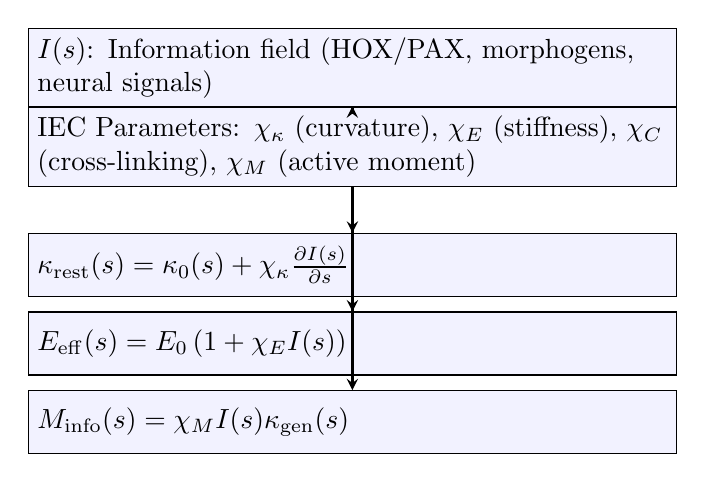
\begin{tikzpicture}[
    node distance=1cm,
    eqbox/.style={rectangle, draw, fill=blue!5, text width=8cm, minimum height=0.8cm, align=left},
    arrow/.style={->, >=stealth, thick}
]

% Information Field
\node[eqbox] (I) {$I(s)$: Information field (HOX/PAX, morphogens, neural signals)};

% IEC Parameters
\node[eqbox, below of=I] (params) {IEC Parameters: $\chi_{\kappa}$ (curvature), $\chi_{E}$ (stiffness), $\chi_{C}$ (cross-linking), $\chi_{M}$ (active moment)};

% Equations
\node[eqbox, below of=params, yshift=-0.5cm] (eq1) {$\kappa_{\mathrm{rest}}(s) = \kappa_{0}(s) + \chi_{\kappa} \frac{\partial I(s)}{\partial s}$};

\node[eqbox, below of=eq1] (eq2) {$E_{\mathrm{eff}}(s) = E_{0} \left(1 + \chi_{E} I(s)\right)$};

\node[eqbox, below of=eq2] (eq3) {$M_{\mathrm{info}}(s) = \chi_{M} I(s) \kappa_{\mathrm{gen}}(s)$};

% Arrows
\draw[arrow] (I) -- (params);
\draw[arrow] (params) -- (eq1);
\draw[arrow] (params) -- (eq2);
\draw[arrow] (params) -- (eq3);

\end{tikzpicture}
\caption{Information-Elasticity Coupling (IEC) equations. The information field $I(s)$ modulates mechanical properties through dimensionless coupling parameters $\chi_{\kappa}$, $\chi_{E}$, $\chi_{C}$, and $\chi_{M}$, producing modified rest curvature, effective stiffness, and active moments.}
\label{fig:iec_equations}
\end{figure}


